\documentclass[a4paper, 12pt]{article}

% Fonts
%\usepackage[default,osfigures,scale=0.95]{opensans}
%\usepackage[T1]{fontenc}
%\usepackage{textcomp}
%\usepackage[varqu,varl]{zi4}% inconsolata typewriter
\usepackage{amsmath,amsthm}
%\usepackage[cmintegrals]{newtxsf}
%\usepackage{ae}

\usepackage{etex}
\usepackage{bm, bbm}
\usepackage{amssymb}
\usepackage{mathtools}
\usepackage{natbib}
\usepackage{epsfig}
\usepackage{pdflscape}
\usepackage{sectsty}
\usepackage{graphicx}
\usepackage[margin=1in, nohead]{geometry}
\usepackage{hyperref}
\usepackage{setspace}
\usepackage{caption}
\captionsetup{font={stretch=.5}}
%\usepackage{authblk}
\usepackage{dcolumn}
%\usepackage{floatrow}
\usepackage{booktabs}
\usepackage{xr}
\usepackage{soul}
\usepackage{calc}
\usepackage{epigraph}
\usepackage{enumitem}
\usepackage{abstract}
\usepackage{pgfplots}
\usepackage{tikz}
\usetikzlibrary{decorations.pathreplacing}
\usetikzlibrary{calc}
\usepackage{footmisc}
\usepackage{titlesec}
\usepackage{array}
\usepackage{placeins}
\newcolumntype{L}[1]{>{\raggedright\let\newline\\\arraybackslash\hspace{0pt}}m{#1}}
\newcolumntype{C}[1]{>{\centering\let\newline\\\arraybackslash\hspace{0pt}}m{#1}}
\newcolumntype{R}[1]{>{\raggedleft\let\newline\\\arraybackslash\hspace{0pt}}m{#1}}
\newcolumntype{d}[1]{D{.}{.}{#1}}

\renewcommand{\abstractname}{}    % clear the title
\renewcommand{\absnamepos}{empty} % originally center

\renewcommand*\rmdefault{ppl}

\setlist[itemize]{leftmargin=*}
\renewcommand{\footnotelayout}{\raggedright}

\titlelabel{\thetitle.\quad}
\titleformat*{\section}{\centering\scshape\large}
\titleformat*{\subsection}{\centering\itshape}
\titleformat{\subsubsection}[runin]{\bfseries}{\thesubsubsection}{1em}{}

\renewcommand{\abstractname}{}
\renewcommand{\absnamepos}{empty}

\graphicspath{{./}}

\DeclarePairedDelimiter{\floor}{\lfloor}{\rfloor}

\hypersetup{
    colorlinks,%
    citecolor=brown,%
    filecolor=blue,%
    linkcolor=blue,%
    urlcolor=black
}

\graphicspath{{figures/}}

\renewcommand{\abstractname}{\vspace{-\baselineskip}}

\DeclareMathOperator*{\argmax}{arg\,max}
\newtheorem{proposition}{Proposition}
\newtheorem{lemma}{Lemma}
\newtheorem{hypothesis}{Hypothesis}
\newtheorem{prediction}{Prediction}
\newtheorem{assumption}{Assumption}
\newtheorem{definition}{Definition}
\newtheorem{remark}{Remark}
\newtheorem{example}{Example}
\newtheorem{corollary}{Corollary}
\DeclareMathOperator{\sign}{sign}

\newcommand{\I}{\mathbbm{1}}
\newcommand{\E}{\mathbbm{E}}
\newcommand{\R}{\mathbbm{R}}

\newcommand{\mc}[2]{\multicolumn{#1}{c}{#2}}
\allsectionsfont{\raggedright\mdseries}\subsectionfont{\raggedright\itshape\mdseries}
 
\usetikzlibrary{fit,positioning}
\usetikzlibrary{decorations.pathreplacing}
\usetikzlibrary{calc}

\begin{document}

\title{{\bf Modeling Asymmetric Relationships from Symmetric Networks}}

\author{
  Arturas Rozenas\\
{\small NYU}\\
  {\small \texttt{ar199@nyu.edu}}
\and
  Shahryar Minhas\\
{\small MSU}\\
  {\small \texttt{minhassh@msu.edu}}
  \and
  John Ahlquist\\
{\small UCSD}\\
  {\small \texttt{jahlquist@ucsd.edu}}
\thanks{Versions of this paper were presented at the 2015 meetings of the International Political Economy Society, the 2016 meetings of the Society for Political Methodology, and WardFest.  We thank James Fowler, Jenn Larson, and Mike Ward for useful comments. Micah Dillard provided excellent research assistance.  Ahlquist benefitted from a fellowship at Stanford's Center for Advanced Study in the Behavioral Sciences during the writing of this paper.  Installation instructions for the P-GBME package and files to replicate the analyses in this paper are available at \url{http://github.com/s7minhas/pgbmeRepl}.}}

\maketitle 
\thispagestyle{empty}

\bigskip

\begin{abstract}
 \noindent Many bilateral relationships requiring mutual agreement produce observable networks that are symmetric (undirected). However, the unobserved, asymmetric (directed) network is frequently the object of scientific interest. We propose a method that probabilistically reconstructs the latent, asymmetric network from the observed, symmetric graph in a regression-based framework. We apply this model to the bilateral investment treaty network. Our approach successfully recovers the true data generating process in simulation studies, extracts new, politically relevant information about the network structure inaccessible to alternative approaches, and has superior predictive performance. 
\end{abstract}

\clearpage

\singlespacing

\section{Introduction} % PA has "Introduction" title for intro section

Social actors are often embedded in webs of relationships that profoundly shape political and economic outcomes \citep{franzese:hays:2008,ward:etal:2011}. One challenge in analyzing networks arises in situations where an analyst cannot fully observe the nature of relational ties. In many dyadic interactions --- treaties, marriages --- outsiders can observe ties only if both agents agree, that is, the payoff for forming a tie exceeds its cost for \emph{both} members of a dyad \citep{jackson:wolinsky:1996}. The observed network is therefore composed of symmetric (``undirected'') ties even though the social process at work contains important relational asymmetries. The pursuit of a tie by one party may not be reciprocated to the same extent by another.

As an illustration, suppose $A$, $B$, and $C$ are three warring factions deciding whether to sign bilateral peace agreements. We observe a network in which dyads $(A, C)$ and $(B, C)$ have signed agreements, but the dyad $(A, B)$ continues fighting. This observed network of `peaceful' ties could be generated from any of  three unobserved sets of relations: it may be that $B$ failed to reciprocate $A$'s pursuit of peace, or vice versa, or neither $A$ nor $B$ pursued peace. To identify conditions that drive factions to sign peace agreements we must account for these unobserved asymmetries.  Here, the observed symmetric graph is an incomplete representation of the underlying, asymmetric network, which is frequently the object of scientific interest.  We refer to this situation as ``partial observability.'' 

%As an illustration, suppose $A$, $B$, and $C$ are three warring factions deciding whether to sign bilateral peace agreements. The left panel of Figure \ref{fig:ntw} shows a network where dyads $(A, C)$ and $(B, C)$ sign agreements, but the dyad $(A, B)$ continues fighting. This observed network of `peaceful' ties could be generated from any of the three unobserved networks shown in the right panel of Figure \ref{fig:ntw}. It may be that $B$ failed to reciprocate $A$'s pursuit of peace, or vice versa. Or neither $A$ nor $B$ wanted peace. In order to effectively identify conditions that drive factions to form peace we must account for these unobserved relational asymmetries.  In other words, the observed symmetric network is only an incomplete representation of the underlying asymmetric network, which is frequently the object of scientific interest.  We refer to this situation as ``partial observability.'' 

% \begin{figure}[h!]

% \begin{tikzpicture}

% \tikzstyle{main}=[circle, minimum size = 0mm, thick, draw =black!80, node distance = 6mm]
% \tikzstyle{box}=[rectangle, draw=black!100]
% \hspace{-.7cm}

%   \node[main] (A) at (0, 2.95) {$A$} { };
%   \node[circle, minimum size = 10mm, draw = white, node distance = 6mm, right = of A] (D) {} { };
%   \node[main] (B) [right = of D] {$B$} { };
%   \node[main] (C) [above = of D] {$C$} {};
% \node[circle, minimum size = 10mm, draw = white, node distance = 0mm, above = of C] (E) {} { };
% \draw[-, thick] (A) -- (C);
% \draw[-, thick] (B) -- (C);
%   \node[circle, minimum size = 10mm, draw = white, node distance = 14.5mm, below = of C] (X) {} { };
%   \node[rectangle, inner sep=4.4mm,draw=black!100, fit= (A) (B) (C) (X) (E)] (R) {};
% \node [above=2.7cm, align=flush center, text width=8cm] at (R) {{\bf Observed network}};     
 
% \node[main] (A) at (5,2) {$A$} { };
%   \node[circle, minimum size = 0mm, draw = white, node distance = 6mm, right = of A] (D) {} { };
%   \node[main] (B) [right = of D] {$B$} { };
%   \node[main] (C) [above = of D] {$C$} {};
% \draw[-latex]  (A) to [bend left] (C);
% \draw[-latex]  (C) to [bend left] (A);
% \draw[-latex]  (C) to [bend left] (B);
% \draw[-latex]  (B) to [bend left] (C);
% \draw[-latex]  (B) to [bend left] (A);

% \node[main] (A1) at (9,2) {$A$} { };
% \node[circle, minimum size = 0mm, draw = white, node distance = 6mm, right = of A1] (D) {} { };
% \node[main] (B1) [right = of D] {$B$} { };
% \node[main] (C1) [above = of D] {$C$} {};
% \draw[-latex]  (A1) to [bend left] (C1);
% \draw[-latex]  (C1) to [bend left] (A1);
% \draw[-latex]  (C1) to [bend left] (B1);
% \draw[-latex]  (B1) to [bend left] (C1);
% \draw[-latex]  (A1) to [bend right] (B1);

% \node[main] (A2) at (7,4.3) {$A$} { };
% \node[circle, minimum size = 0mm, draw = white, node distance = 6mm, right = of A2] (D) {} { };
% \node[main] (B2) [right = of D] {$B$} { };
% \node[main] (C2) [above = of D] {$C$} {};
% \draw[-latex]  (A2) to [bend left] (C2);
% \draw[-latex]  (C2) to [bend left] (A2);
% \draw[-latex]  (C2) to [bend left] (B2);
% \draw[-latex]  (B2) to [bend left] (C2);


% \node[rectangle, inner sep=4.4mm,draw=black!100, fit= (A) (B) (C) (A1) (B1) (C1) (A2) (B2) (C2)] (R) {};
%              \node [above=2.75cm, align=flush center ,text width=8cm] at (R) {{\bf Possible unobserved networks}};     
% \end{tikzpicture}

% \caption{The observed undirected network in the left panel is consistent with any of the three directed networks in the right panel, which cannot be observed.}
% \label{fig:ntw}
% \end{figure}

We present the partial observability generalized bilinear mixed effects model (P-GBME) to address this challenge.  The model is a synthesis of the generalized bilinear mixed effects (GBME) model \citep{hoff:2005} and the bivariate or ``partial observability'' probit model \citep{poirier:1980, przeworski:vreel:2002}. The model can probabilistically reconstruct the directed network from which the observed, undirected graph emerged. The model enables the study of network ties in a regression framework by accounting for interdependencies as well as unobserved asymmetries in network relations. The stochastic actor-oriented model (SAOM) for networks \citep{snijders:pickup:2017, stadtfeld:etal:2017} also allows for partial observability. However, SAOM was designed to assess how specific network features (e.g., $k$-star triangles) give rise to an observed network. The latent network approach is not used to study the role of specific network statistics.  Rather, latent network models aim to account for broad patterns of network interdependence using a variance decomposition regression framework.\footnote{See \citet{minhas:etal:2016:arxiv} for detailed discussion. Other approaches based on generalized spatio-temporal dependence can also recover directed predicted probabilities \citet{franzese:etal:2012}.}

We illustrate the P-GBME model by applying it to the bilateral investment treaties (BIT) network for each year in 1990-2012. The model substantially improves predictive accuracy relative to both conventional logit and standard GBME. As important, P-GBME extracts new information about the factors that drive treaty preferences, identifies important structural changes in the network, and highlights possible ``hidden'' agreements that are easily overlooked when latent network asymmetries are ignored.

\section{The Model}

Building on the random utility framework \citep{mcfadden:1980}, we model an actor $i = 1, \ldots,  N$ as having net utility from forming a tie with another $j$: $z_{ij} = \mu_{ij} + \epsilon_{ij}$ with $\mu_{ij}$ representing the systematic component (that depends on observables) and $\epsilon_{ij}$ representing the stochastic error. To account for interdependencies in actors' utilities from having ties, we use the ``latent space'' approach \citep{hoff:2005} and model these utilities as follows:
\begin{align}    
\left ( \begin{array}{c}
         z_{ij} \\
         z_{ji} \end{array} \right ) 
         & \sim \mathcal{N}
        \left ( \begin{array}{c}
         \mu_{ij} + a_i + b_j +    \bm{u}'_i\bm{v}_j  \\
         \mu_{ji} + a_j + b_i +  \bm{u}'_j\bm{v}_i \end{array}, \left [ \begin{array}{cc}
        \sigma^2 & \rho \sigma^2 \\
         \rho \sigma^2 & \sigma^2 \end{array} \right] \right ). \label{eq:modz}
\end{align}
The correlation, $\rho$, captures the ``reciprocity'' between the utilities that actors derive from tie formation. Parameters $a_i$ and $b_j$ are sender- and receiver-specific random effects, respectively, and they capture second-order network dependencies. The vectors $\bm{u}_i$ and $\bm{v}_i$ represent the location of actor $i$ in the latent space of `senders' and `receivers,' respectively. These random effects capture higher-order dependencies in network ties: $i$ derives a large utility from forming a tie with $j$, if $i$'s location in the latent space of `senders' $\bm{u}_i$ is close to $j$'s location in the latent space of `receivers' $\bm{u}_j$ (so that the cross-product $\bm{u}'_i\bm{v}_j$ is large).\footnote{As in previous literature, these random effects are modeled as $(a_i, b_i) \sim \mathcal{N}(0, \bm{\Sigma_{ab}})$, $\bm{u}_i \sim \mathcal{N}_K(\bm{0}, \sigma_u^2\bm{I})$, and $\bm{v}_i \sim \mathcal{N}_K(\bm{0}, \sigma_v^2\bm{I})$, where $\bm{\Sigma_{ab}}$, $\sigma_u^2$, and $\sigma_v^2$ are unknown parameters. The choice of $K$, dimensionality of the latent space, is discussed supplementary materials.} We express the systematic components of actors' utilities as linear functions of predictors:
\begin{align}
    \mu_{ij} & = \bm{\beta}^{(s)}\bm{x}_i^{(s)} + \bm{\beta}^{(r)}\bm{x}_j^{(r)} + \bm{\beta}^{(d)}\bm{x}_{ij}^{(d)}, \label{eq:itoj}\\
    \mu_{ji} & = \bm{\beta}^{(s)}\bm{x}_j^{(s)} + \bm{\beta}^{(r)}\bm{x}_i^{(r)} + \bm{\beta}^{(d)}\bm{x}_{ji}^{(d)} \label{eq:jtoi}.
\end{align}

A researcher cannot directly observe net utility (the $z$'s).  We only observe agents' behaviors, in this case undirected \emph{bilateral} ties. A directional tie $i \to j$ is formed if and only if $i$'s net gain from doing so is strictly positive, $z_{ij} > 0$.  Accordingly, the bilateral tie $i \leftrightarrow j$ is formed if and only if \emph{both} actors derive a net positive payoff from having a tie so that $z_{ij} > 0$ and $z_{ji} > 0$. A researcher observes an undirected (bilateral) tie $y_{ij} = y_{ji} = \{0, 1\}$ arising from the following data generating process:
\begin{align}
y_{ij} = y_{ji} & =   \left\{ \begin{array}{ll}
         1 & \mbox{if $z_{ij} > 0$ and $z_{ji} > 0$},\\
         0 & \mbox{else}.\end{array} \right. \label{mod:y}
\end{align}

Under a standard identifying restriction $\sigma^2 = 1$, the model is a partially observable probit regression \citep{poirier:1980}, augmented with random-effects to capture unobserved heterogeneity and inter-dyadic dependencies. Vectors $\bm{x}_i^{(s)}$ and $\bm{x}_i^{(r)}$ represent the sender-specific and receiver-specific covariates, respectively. A model for the directional link $i \to j$ (eq. \ref{eq:itoj}), uses variables $\bm{x}_i$ as sender-specific predictors, but these same predictors become receiver-specific in the model for the directional link $j \to i$ (eq. \ref{eq:jtoi}). Vector $\bm{x}_{ij}^{(d)}$ contains dyad-specific variables. These dyad-specific variables might be symmetric, $x_{ij} = x_{ji}$ (e.g., distance between countries), or not (e.g., export-import).

A partially observed probit model requires at least one of the following identifying restrictions: (1) regression equations \ref{eq:itoj} and \ref{eq:jtoi} must have the same parameters and/or (2) one equation contains a predictor not included in another equation \citep{poirier:1980}. If the dyadic predictors are asymmetric, $\bm{x}_{ij} \neq \bm{x}_{ji}$, then condition (2) is satisfied. Furthermore, regression equations \ref{eq:itoj} and \ref{eq:jtoi} have the same parameters, and so condition (1) holds as well; thus, the above model is parametrically identified. However, we impose an additional restriction that $\rho = 0$. While this restriction is not required for parametric identification, \citet{rajbhandari:2014} showed that finite sample estimates of $\rho$ are sensitive to the starting values and generally cannot be treated as reliable.\footnote{The estimation algorithm provided with this paper allows $\rho$ to be estimated, but caution should be used when utilizing this option.}
 
We estimate the model in a Bayesian framework using Markov chain Monte Carlo.  In the supplemental materials give a more detailed exposition of the model, prior assumptions, the sampling algorithm. We also provide results from a simulation study demonstrating that the model successfully recovers known parameter values.
\section{Application: Bilateral Investment Treaties}

We apply the P-GBME model to the network of bilateral investment treaties (BITs) from 1990 to 2012 using the standard United Nations BIT database. There is a vibrant debate on whether BITs boost FDI \citep{jandhyala:etal:2011, simmons:2014,minhas:2016}, but a proper resolution of this debate requires a convincing empirical model of treaty formation \citep{rosendorff:shin:2012}. Partial observability is one key challenge in building such model: the observed network of signed bilateral treaties is symmetric, while the underlying preferences for these treaties are  asymmetric. 

We fit the P-GBME model separately for each year of data using a suite of covariates that closely follows  the existing empirical literature (see supplementary materials). Our model improves on the previous literature by accounting for both network interdependence and partial observability. 

\subsection{Predictive Performance}

In Table~\ref{tab:perfAssess} we compare the in-sample and out-of-sample predictive performance of the P-GBME to that of pooled probit, which assumes dyadic independence and ignores partial observability, and GBME, which models dyadic interdependencies, but not partial observability. The predictive accuracy of the GBME model in this case is similar to the pooled probit. Adding the partial observability component to the GBME model, however, produces an additional substantial improvement in the predictive accuracy as shown by all metrics for the P-GBME model.

\begin{table}[h!]
\centering
\begin{tabular}{lcccccc}
\toprule
& & \multicolumn{2}{c}{In-sample} & & \multicolumn{2}{c}{Out-of-sample} \\
\cmidrule{3-4}\cmidrule{6-7}
& & ROC & PR & & ROC & PR\\
\midrule
Pooled probit& & 0.75 & 0.48 &  & 0.73 & 0.44\\
GBME && 0.76 & 0.47 & & 0.77 & 0.48 \\
P-GBME && 0.90 & 0.71 & & 0.91 & 0.78 \\
\bottomrule
\end{tabular}
\caption{Predictive performance in BIT data: area under the receiver operating characteristic curve (ROC) and area under the precision recall curve (PR).}
\label{tab:perfAssess}
\end{table} 

\subsection{Regression Parameters}

Existing models, including GBME, estimate a single coefficient for each predictor. This assumes away the possibility that the same factor differentially ``affects'' $i$'s demand for a treaty with $j$ and $i$'s attractiveness to $j$.  The P-GBME recovers directed sender- and receiver-effects for node-level covariates. For instance, our estimates suggest that, countries faster growth in GDP per capita were no more inclined to sign BITs with others (sender effect).  But high-growth countries were more attractive BIT partners to others (receiver effect). Supplementary materials describes regression parameter estimates in detail.

\subsection{The Structure of Latent Treaty Preferences}

The P-GBME model allows us to extract ``latent preferences'' for treaty formation -- the estimated probability that country $i$ demands a treaty from $j$, and vice versa. Figure~\ref{fig:predplotCHN} displays the mean posterior predicted probabilities relevant to China in 1995 and 2010. The horizontal axis represents a country's attractiveness to China as a BIT partner and the vertical axis is China's attractiveness to that country. Countries above the diagonal line find China a more attractive BIT partner than China finds them, and vice versa.  Color identifies observed BITs.

The plots reveal how China's position in the BIT network changed over time. In 1995, China was moving aggressively to demand BITs around the world, forming ties that the model views as relatively unlikely. By 2010, China had many more BITs in place and is more likely to be a treaty target by the remaining countries, an indication of China's expanded role in the global economy.  

\begin{figure}[ht]
	\centering
	\begin{tabular}{cc}
		1995 & 2010 \\
		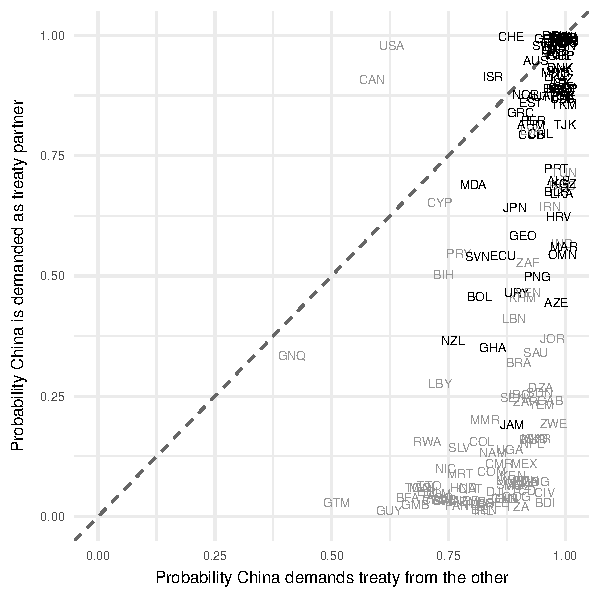
\includegraphics[width=.4\textwidth]{figure1_a.pdf} & 
		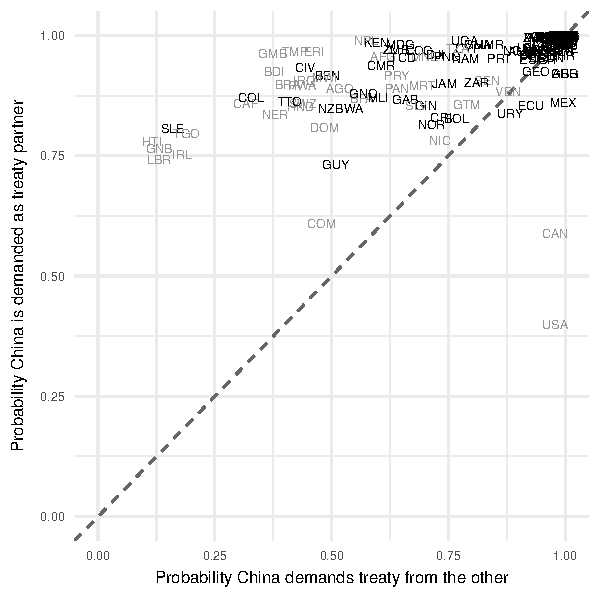
\includegraphics[width=.4\textwidth]{figure1_b.pdf} \\
	\end{tabular}
	\caption{Each panels displays the posterior mean probability that China demands and will be demanded as a BIT partner. Country labels in black designate those that had formed a BIT with China by the specified year.}	
	\label{fig:predplotCHN}
\end{figure}
\FloatBarrier

Figure~\ref{fig:predplotUSA} illustrates a different use of the P-GBME model.  It shows the predicted probabilities that the USA is demanded (left) and demands (right) a BIT in 2010.  Observe that the model predicts Peru, Mexico, and Chile---the top 3 non-BITs---demand a BIT with the USA at probabilities close to one, and are also likely BIT targets of the USA with probabilities exceeding $0.5$. Closer inspection of UN treaty data reveals that, by 2010, all three had signed other agreements with the US that contain provisions functionally equivalent to BITs; these agreements do not appear in the BIT dataset commonly used in the literature.\footnote{The treaties are 2006 Peru-USA Free Trade Agreement (FTA), NAFTA in 1992, and the 2003 Chile-USA FTA. These agreements included investment provisions that mirror the terms of a BIT almost exactly (see \url{http://investmentpolicyhub.unctad.org/Download/TreatyFile/5454}).} The P-GBME model nevertheless highlights these ``hidden'' agreements as dyads likely to have a BIT. This suggests that researchers studying BITs need to carefully examine the dataset they employ and perhaps expand the set of treaties considered relevant.

\begin{figure}[ht]
	\centering
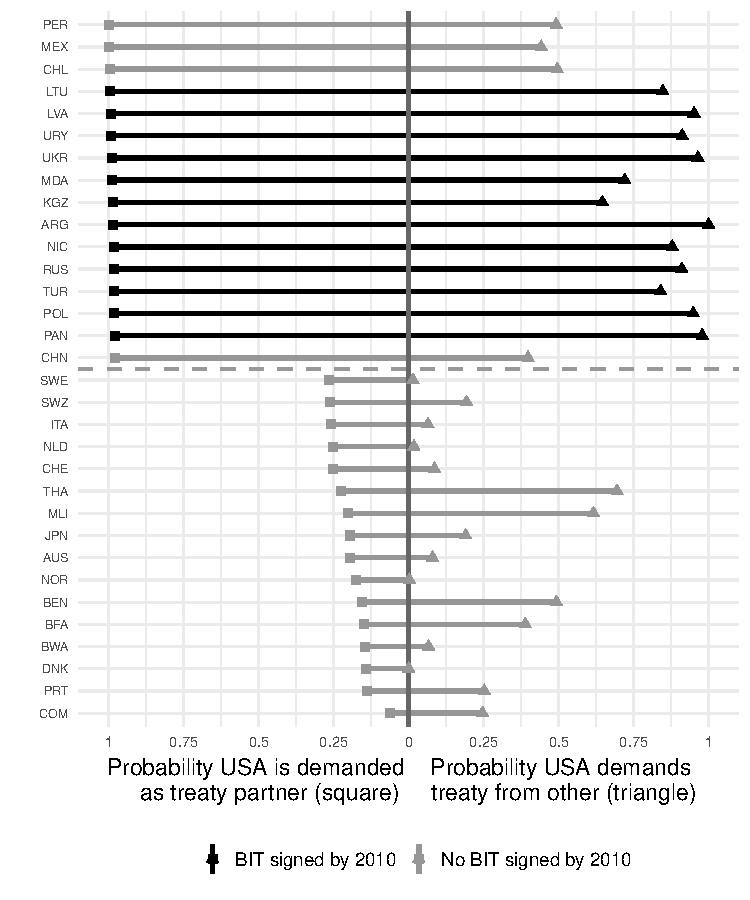
\includegraphics[width=.7\textwidth]{figure2.pdf} 
\caption{The posterior probability a country demands a BIT (left) and is demanded (right) with the USA in 2010 (the top and bottom decile of countries).  P-GBME is good at separating likely from unlikely treaties as well as identifying ``hidden agreements.''}	
	\label{fig:predplotUSA}
\end{figure}
\FloatBarrier

\section{Conclusion}

Partial observability occurs whenever the observed graph is undirected yet the underlying process implies directed relationships. We introduced a model that can reconstruct the latent directed network ties, and illustrated its advantages on an example of bilateral trade agreements. The future work in this area could focus on several extensions. First, we accounted for network dependencies using bilinear mixed effects framework (GBME), which could be generalized using  the recently developed additive and multiplicative effects network model \citep{hoff:2015:arxiv,minhas:etal:2016:arxiv}. Second, estimating this type of network model in a fully dynamic setting (as opposed to slicing data by time, as we did here) remains a challenge, especially when the set of nodes changes in time.

%\clearpage
\singlespacing
\bibliographystyle{apsr}
\bibliography{master}


\end{document}